\documentclass[runningheads,a4paper]{llncs}
\usepackage[T1]{fontenc}
\usepackage{booktabs,graphicx,amsmath,url,xurl}
\usepackage{tikz}
\usetikzlibrary{arrows.meta,positioning}
\setlength{\emergencystretch}{2em}
\begin{document}
\title{Compiler-Guided Proof Repair in Lean 4:\\Controlled Local-Model Pilots and Negative Evidence}
\titlerunning{Controlled Lean 4 Proof Repair Pilots}
\author{Anonymous author}\authorrunning{Anonymous author}
\institute{Affiliation withheld for review}
\maketitle
\begin{abstract}
Do Lean 4 compiler diagnostics improve strict proof verification over equally
budgeted retries? We report two distinct local-model studies, not a pooled
benchmark. In the original fixed-theorem pilot (60 test types, one quantized
Qwen2.5-7B model), one-shot and blind retry verify 0/60 and 1/60 targets;
guided repair verifies 1/58 observed targets, with two outcomes unavailable.
The 58 complete pairs solve the same single target. In a separately constructed,
post-hoc follow-up (24 elementary types, three seeds), guided repair verifies
10/72 versus 5/72 for neutral retry but 9/72 for shuffled diagnostics.
A coding-specialized Qwen2.5-7B follow-up verifies 11/72 with or without
correct diagnostics and 14/72 with independent resampling. Exploratory
family-bootstrap intervals fail to establish diagnostic-specific superiority.
Strict proof checking, repetition and feedback-content controls are distinguished
from natural-language semantic fidelity. Discovered theorem-family overlaps
and AI-review flags constrain benchmark independence. These results support an
auditable negative/inconclusive comparison, not an improved prover or an
end-to-end NL-to-Lean accuracy claim.
\keywords{Lean 4 \and proof repair \and compiler diagnostics \and controlled inference \and negative results}
\end{abstract}

\section{Question and Prior Work}
A proof can change its text, eliminate a compiler error, or prove the supplied
Lean theorem. Only the last is the primary outcome. Even that outcome does not
establish that a formal type preserves an English mathematical statement.
We ask whether providing diagnostics from a failed candidate helps a small
local model more than another generation opportunity with no diagnostics.
The control must keep the theorem and initial candidate fixed and record
actual input costs, because feedback increases context length.

Lean 4 and Mathlib provide kernel-checked proof infrastructure
\cite{lean4,mathlib}. miniF2F and LeanDojo examine other formal-proving
settings \cite{minif2f,leandojo}. ProofNet illustrates the distinct
natural-language formalization problem \cite{proofnet}. Baldur and APRIL
study learned or supervised proof repair \cite{baldur,april}; Li and Li
analyse the role of verifier feedback relative to resampling
\cite{hindsight}. We do not claim priority for guided repair, blind retry,
or feedback controls. Our contribution is a small-model, explicit-comparator
study, including low-signal and adverse findings, not a new repair algorithm.

\section{Design, Scope and Verification}
\textbf{Original pilot (Study~1).} Sixty fixed Lean theorem types were evaluated
with a single hash-pinned 4-bit Qwen2.5-7B-Instruct model. A generated one
candidate; B and C shared that candidate and received up to three further
calls. B used blind feedback, C the real Lean diagnostics. Strict verification
required an exact expected theorem type and no admitted proof shortcuts.
The initial experiment used one seed and full Mathlib; two guided trajectories
were unavailable. It did \emph{not} evaluate autonomous English-to-Lean translation.
Reference review was AI-assisted, not independent human gold annotation.

\textbf{Constructed follow-up (Study~2).} A separate, elementary 24-type Lean
benchmark used a narrower, fixed-import environment and three seeds (2027,
2028, 2029). Twelve development types were used for calibration, with
V5 development and V7 test protocols separately versioned; a test-only
source-spacing correction to $t08$ was made during reference screening,
before model inference. V7 evaluated the base model under B (neutral), C
(correct diagnostics), D (shuffled diagnostics), E (token-matched neutral),
and R (independent resampling), each with up to three repairs. All five
arms shared the same initial within each theorem--seed evaluation; condition
random streams were separated and arm order rotated. V8 subsequently applied
the same constructed test cohort and seeds to a coding-specialized 4-bit
Qwen2.5-Coder-7B model in a separately recorded run. V8 is exploratory
relative to the already inspected base-model evidence. V9's novel repair
prompt was assessed on development only and not promoted to a new confirmatory
test. Neither follow-up evaluates end-to-end NL-to-Lean faithfulness: its
English descriptions are synthetic placeholders.

\begin{figure}[t]
\centering
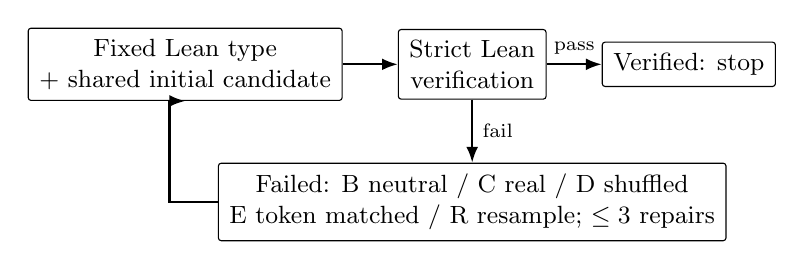
\begin{tikzpicture}[font=\small,node distance=5mm and 7mm,
 every node/.style={align=center},
 bx/.style={draw,rounded corners=1pt,inner sep=4pt},
 arr/.style={-{Latex[length=2mm]},thick}]
\node[bx] (type) {Fixed Lean type\\+ shared initial candidate};
\node[bx,right=of type] (check) {Strict Lean\\verification};
\node[bx,right=of check] (pass) {Verified: stop};
\node[bx,below=8mm of check] (repair) {Failed: B neutral / C real / D shuffled\\E token matched / R resample; $\leq3$ repairs};
\draw[arr] (type)--(check);
\draw[arr] (check)--node[above,font=\scriptsize]{pass}(pass);
\draw[arr] (check)--node[right,font=\scriptsize]{fail}(repair);
\draw[arr] (repair.west)-|([xshift=-2mm]type.south)--(type.south);
\end{tikzpicture}
\caption{The Study~2 arms receive the same initial candidate; only C gets its
correct diagnostic. Study~1 used A/B/C; Study~2 is separately versioned.}
\label{fig:workflow}
\end{figure}

\section{Results}
\begin{table}[t]\centering\small
\caption{Study~1 strict verification (original 60 fixed types). C has two unavailable outcomes; the 58 complete B/C pairs each solve the same single target.}
\label{tab:study1}
\begin{tabular}{llll}\toprule
Condition & Verified & Observed denominator & Missing \\
\midrule
A: one-shot & 0 & 60 & 0 \\
B: blind repair & 1 & 60 & 0 \\
C: compiler-guided repair & 1 & 58 & 2 \\
B/C complete pairs & 1 / 1 & 58 & 0 \\
\bottomrule\end{tabular}
\end{table}

\textbf{Original pilot.} A verifies 0/60, B 1/60, and C 1/58 observed,
with two unavailable C outcomes. On the 58 complete B/C pairs, both
arms verify 1/58 and solve the same target; the paired difference is zero,
with no discordant pairs. This is a floor effect, not evidence of
method equivalence. Across all 60, missing-outcome sensitivity allows a
C-minus-B difference from 0 to +3.33 percentage points. On complete
pairs, guided prompts consumed approximately 4353.5 versus 1980.9 mean
input tokens per target for blind repair. Byte-identical retries in the
exploratory post-hoc analysis were 70/172 (40.7\%) under C versus 90/178
(50.6\%) under B; no extra verified theorem resulted. The development
placebo did not establish content-specific comprehension. In the only
jointly verified target (\texttt{lib\_a\_exp\_add}), both branches removed
a reference to the unavailable \texttt{Real.ofReal} constant; the blind
branch succeeded without seeing that diagnostic. This supports neither a
content-specific explanation nor a general success advantage.

\begin{table}[t]\centering\small
\caption{Separate Study~2 strict verification results. Each model has 24
constructed types $\times$ three seeds = 72 repeated theorem--seed observations.
Columns are terminal verification counts, not independent theorem samples.}
\label{tab:study2}
\begin{tabular}{lrrrrrr}\toprule
Model & A & B & C & D & E & R\\\midrule
Qwen2.5-7B base (V7) &4&5&10&9&5&5\\
Qwen2.5-Coder-7B (V8) &11&11&11&11&11&14\\
\bottomrule\end{tabular}
\end{table}

\textbf{Constructed follow-up.} Table~\ref{tab:study2} reports complete
test-cell counts. For the base model, C--B = $+5/72$ (+6.94 points), but
C--D = $+1/72$ (+1.39 points). Exploratory family-cluster bootstrap
95\% intervals are $[-1.67,+15.39]$ and $[-2.78,+6.41]$ percentage points,
respectively; both include zero, and only eight problem families exist.
Because the same theorem types recur across three seeds, 72 is not an
independent-problem denominator for confirmatory tests. Coder's initial
11/72 were not improved by B, C, D or E; R reaches 14/72. Hence the
second model does not establish a diagnostic-specific benefit. In a
subsequent V9 development-only check, an error-aware strategy and the
Coder guided baseline both verified 5/12; this was not used to retune
reported test results.

\begin{table}[t]\centering\small
\caption{Post-hoc sensitivity to discovered construction overlap, V7 base
model only. Results are fixed-record exclusions, not new trials.}
\label{tab:sensitivity}
\begin{tabular}{p{0.52\linewidth}rrrr}\toprule
Cohort & $N$ & B & C & D\\\midrule
All types (original reported cohort) &72&5&10&9\\
Exclude $t11,t12$ (duplicate of development $d06$) &66&5&10&9\\
Also exclude $t13$ (related to development $d07$) &63&5&10&9\\
Also collapse successor pair by excluding $t08$ &60&5&10&9\\
\bottomrule\end{tabular}
\end{table}

\begin{table}[t]\centering\small
\caption{First-generation failure categories in the V7 constructed follow-up
(68 failures; four initial successes). Categories are heuristic compiler labels.}
\begin{tabular}{lrrrr}\toprule
Category & Syntax & Type/elaboration & Unknown name & Other \\
\midrule
Count & 58 & 7 & 2 & 1 \\
\bottomrule\end{tabular}
\end{table}

\section{Benchmark Validity and Threats}
All 24 constructed reference proofs passed fresh strict Lean screening;
40 frozen V8 evidence entries passed the local SHA-256 manifest check.
An automated independent-model review produced 24 records, including
nine duplicate-related flags; these are \emph{not} independent expert
approval. Heuristic comparisons raised 12 within-test and 10
cross-split similarities. Further manual mathematical examination found
an exact development/test Nat binomial-square equivalence ($d06$ versus
$t11,t12$), test $t11/t12$ equivalence, a development $d07$ specialization
of test $t13$, and a related successor pair $t07/t08$. The first three
are especially relevant to independent family separation. Proposed
adjudications are recorded as provisional, not final sign-off.

Table~\ref{tab:sensitivity} holds the recorded model outcomes constant
while removing selected overlaps. The raw C--B and C--D count differences
stay five and one respectively, but denominators and rates change. This
is explicitly post-hoc and does not re-establish a pristine test split.
Such exclusions are not licensed to replace the original results.
Training-set contamination remains unknown. Prompt lengths, limited
coding knowledge, a small model, repeated failed candidates, and the
narrower Study~2 Lean imports further limit attribution. Formal proof
acceptance is not validation of English-to-Lean meaning, nor is the
constructed benchmark a substitute for the original fixed-type study.

\section{Reproducibility and Conclusion}
Study~1 preserved its separate frozen 60-type records. Study~2 V7
provides processed calls, outcomes and transitions, a frozen plan and
script in \url{https://github.com/sadiapeerzada/NLP-to-Formal-Language-Proof}.
V8's locally locked report records a second-model evaluation and AI
review; full raw inference/reviewer journals are not in this manuscript
snapshot, so independent re-execution is not asserted. Neither synthetic
English descriptions nor unadjudicated duplicates can support a claim
of natural-language semantic fidelity. The current package is prepared
for supervisor review, not an approved final public benchmark release.

Across the observed studies, changing feedback can affect candidate
behaviour without establishing additional strict verification relative
to the closest controls. The original paired study has an extreme floor;
the base follow-up's apparent C--B increase is nearly matched by
shuffled feedback, and the Coder follow-up gains nothing from C over
its own initial generation. We therefore report a measured
negative/inconclusive result, retain all original denominators, and
avoid claims of general compiler-feedback superiority or equivalence.

\begin{thebibliography}{10}\small
\bibitem{lean4} de Moura, L., Ullrich, S.: The Lean 4 theorem prover and programming language. CADE (2021).
\bibitem{mathlib} The mathlib Community: The Lean mathematical library. CPP (2020).
\bibitem{minif2f} Zheng, K., Han, J.M., Polu, S.: miniF2F: A cross-system benchmark for formal olympiad-level mathematics. ICLR (2022).
\bibitem{leandojo} Yang, K., et al.: LeanDojo: Theorem proving with retrieval-augmented language models. NeurIPS (2023).
\bibitem{proofnet} Azerbayev, Z., et al.: ProofNet: Autoformalizing and formally proving undergraduate-level mathematics. (2023), arXiv:2302.12433.
\bibitem{baldur} First, E., et al.: Baldur: Whole-proof generation and repair with large language models. ESEC/FSE (2023).
\bibitem{april} Wang, E., et al.: Learning to repair Lean proofs from compiler feedback. arXiv:2602.02990v1 (2026).
\bibitem{hindsight} Li, J., Li, S.: Repair, retry, and the cost of hindsight: Verifier feedback in formal theorem proving. arXiv:2610.22698 (2026).
\end{thebibliography}
\end{document}